%% bare_jrnl_compsoc.tex
%% V1.4b
%% 2015/08/26
%% by Michael Shell
%% See:
%% http://www.michaelshell.org/
%% for current contact information.
%%
%% This is a skeleton file demonstrating the use of IEEEtran.cls
%% (requires IEEEtran.cls version 1.8b or later) with an IEEE
%% Computer Society journal paper.
%%
%% Support sites:
%% http://www.michaelshell.org/tex/ieeetran/
%% http://www.ctan.org/pkg/ieeetran
%% and
%% http://www.ieee.org/

%%*************************************************************************
%% Legal Notice:
%% This code is offered as-is without any warranty either expressed or
%% implied; without even the implied warranty of MERCHANTABILITY or
%% FITNESS FOR A PARTICULAR PURPOSE! 
%% User assumes all risk.
%% In no event shall the IEEE or any contributor to this code be liable for
%% any damages or losses, including, but not limited to, incidental,
%% consequential, or any other damages, resulting from the use or misuse
%% of any information contained here.
%%
%% All comments are the opinions of their respective authors and are not
%% necessarily endorsed by the IEEE.
%%
%% This work is distributed under the LaTeX Project Public License (LPPL)
%% ( http://www.latex-project.org/ ) version 1.3, and may be freely used,
%% distributed and modified. A copy of the LPPL, version 1.3, is included
%% in the base LaTeX documentation of all distributions of LaTeX released
%% 2003/12/01 or later.
%% Retain all contribution notices and credits.
%% ** Modified files should be clearly indicated as such, including  **
%% ** renaming them and changing author support contact information. **
%%*************************************************************************


% *** Authors should verify (and, if needed, correct) their LaTeX system  ***
% *** with the testflow diagnostic prior to trusting their LaTeX platform ***
% *** with production work. The IEEE's font choices and paper sizes can   ***
% *** trigger bugs that do not appear when using other class files.       ***                          ***
% The testflow support page is at:
% http://www.michaelshell.org/tex/testflow/

\documentclass[compsoc,journal,letterpaper,10pt,draftclsnofoot,onecolumn]{IEEEtran}
%
% If IEEEtran.cls has not been installed into the LaTeX system files,
% manually specify the path to it like:
% \documentclass[10pt,journal,compsoc]{../sty/IEEEtran}


% *** MISC UTILITY PACKAGES ***
%
%\usepackage{ifpdf}
% Heiko Oberdiek's ifpdf.sty is very useful if you need conditional
% compilation based on whether the output is pdf or dvi.
% usage:
% \ifpdf
%   % pdf code
% \else
%   % dvi code
% \fi
% The latest version of ifpdf.sty can be obtained from:
% http://www.ctan.org/pkg/ifpdf
% Also, note that IEEEtran.cls V1.7 and later provides a builtin
% \ifCLASSINFOpdf conditional that works the same way.
% When switching from latex to pdflatex and vice-versa, the compiler may
% have to be run twice to clear warning/error messages.






% *** CITATION PACKAGES ***
%
\ifCLASSOPTIONcompsoc
  % IEEE Computer Society needs nocompress option
  % requires cite.sty v4.0 or later (November 2003)
  \usepackage[nocompress]{cite}
\else
  % normal IEEE
  \usepackage{cite}
\fi
% cite.sty was written by Donald Arseneau
% V1.6 and later of IEEEtran pre-defines the format of the cite.sty package
% \cite{} output to follow that of the IEEE. Loading the cite package will
% result in citation numbers being automatically sorted and properly
% "compressed/ranged". e.g., [1], [9], [2], [7], [5], [6] without using
% cite.sty will become [1], [2], [5]--[7], [9] using cite.sty. cite.sty's
% \cite will automatically add leading space, if needed. Use cite.sty's
% noadjust option (cite.sty V3.8 and later) if you want to turn this off
% such as if a citation ever needs to be enclosed in parenthesis.
% cite.sty is already installed on most LaTeX systems. Be sure and use
% version 5.0 (2009-03-20) and later if using hyperref.sty.
% The latest version can be obtained at:
% http://www.ctan.org/pkg/cite
% The documentation is contained in the cite.sty file itself.
%
% Note that some packages require special options to format as the Computer
% Society requires. In particular, Computer Society  papers do not use
% compressed citation ranges as is done in typical IEEE papers
% (e.g., [1]-[4]). Instead, they list every citation separately in order
% (e.g., [1], [2], [3], [4]). To get the latter we need to load the cite
% package with the nocompress option which is supported by cite.sty v4.0
% and later. Note also the use of a CLASSOPTION conditional provided by
% IEEEtran.cls V1.7 and later.





% *** GRAPHICS RELATED PACKAGES ***
%
\ifCLASSINFOpdf
   \usepackage[pdftex]{graphicx}
  % declare the path(s) where your graphic files are
   \graphicspath{{../media/}}
  % and their extensions so you won't have to specify these with
  % every instance of \includegraphics
  \DeclareGraphicsExtensions{.pdf,.jpeg,.png}
\else
  % or other class option (dvipsone, dvipdf, if not using dvips). graphicx
  % will default to the driver specified in the system graphics.cfg if no
  % driver is specified.
  \usepackage[dvips]{graphicx}
  % declare the path(s) where your graphic files are
  \graphicspath{{../media/}}
  % and their extensions so you won't have to specify these with
  % every instance of \includegraphics
  \DeclareGraphicsExtensions{.eps}
\fi
% graphicx was written by David Carlisle and Sebastian Rahtz. It is
% required if you want graphics, photos, etc. graphicx.sty is already
% installed on most LaTeX systems. The latest version and documentation
% can be obtained at: 
% http://www.ctan.org/pkg/graphicx
% Another good source of documentation is "Using Imported Graphics in
% LaTeX2e" by Keith Reckdahl which can be found at:
% http://www.ctan.org/pkg/epslatex
%
% latex, and pdflatex in dvi mode, support graphics in encapsulated
% postscript (.eps) format. pdflatex in pdf mode supports graphics
% in .pdf, .jpeg, .png and .mps (metapost) formats. Users should ensure
% that all non-photo figures use a vector format (.eps, .pdf, .mps) and
% not a bitmapped formats (.jpeg, .png). The IEEE frowns on bitmapped formats
% which can result in "jaggedy"/blurry rendering of lines and letters as
% well as large increases in file sizes.
%
% You can find documentation about the pdfTeX application at:
% http://www.tug.org/applications/pdftex






% *** MATH PACKAGES ***
%
\usepackage{amsmath}
% A popular package from the American Mathematical Society that provides
% many useful and powerful commands for dealing with mathematics.
%
% Note that the amsmath package sets \interdisplaylinepenalty to 10000
% thus preventing page breaks from occurring within multiline equations. Use:
\interdisplaylinepenalty=2500
% after loading amsmath to restore such page breaks as IEEEtran.cls normally
% does. amsmath.sty is already installed on most LaTeX systems. The latest
% version and documentation can be obtained at:
% http://www.ctan.org/pkg/amsmath

\usepackage{amssymb}



% *** SPECIALIZED LIST PACKAGES ***
%
%\usepackage{algorithmic}
% algorithmic.sty was written by Peter Williams and Rogerio Brito.
% This package provides an algorithmic environment fo describing algorithms.
% You can use the algorithmic environment in-text or within a figure
% environment to provide for a floating algorithm. Do NOT use the algorithm
% floating environment provided by algorithm.sty (by the same authors) or
% algorithm2e.sty (by Christophe Fiorio) as the IEEE does not use dedicated
% algorithm float types and packages that provide these will not provide
% correct IEEE style captions. The latest version and documentation of
% algorithmic.sty can be obtained at:
% http://www.ctan.org/pkg/algorithms
% Also of interest may be the (relatively newer and more customizable)
% algorithmicx.sty package by Szasz Janos:
% http://www.ctan.org/pkg/algorithmicx




% *** ALIGNMENT PACKAGES ***
%
\usepackage{array}
% Frank Mittelbach's and David Carlisle's array.sty patches and improves
% the standard LaTeX2e array and tabular environments to provide better
% appearance and additional user controls. As the default LaTeX2e table
% generation code is lacking to the point of almost being broken with
% respect to the quality of the end results, all users are strongly
% advised to use an enhanced (at the very least that provided by array.sty)
% set of table tools. array.sty is already installed on most systems. The
% latest version and documentation can be obtained at:
% http://www.ctan.org/pkg/array


% IEEEtran contains the IEEEeqnarray family of commands that can be used to
% generate multiline equations as well as matrices, tables, etc., of high
% quality.




% *** SUBFIGURE PACKAGES ***
\ifCLASSOPTIONcompsoc
  \usepackage[caption=false,font=footnotesize,labelfont=sf,textfont=sf]{subfig}
\else
  \usepackage[caption=false,font=footnotesize]{subfig}
\fi
% subfig.sty, written by Steven Douglas Cochran, is the modern replacement
% for subfigure.sty, the latter of which is no longer maintained and is
% incompatible with some LaTeX packages including fixltx2e. However,
% subfig.sty requires and automatically loads Axel Sommerfeldt's caption.sty
% which will override IEEEtran.cls' handling of captions and this will result
% in non-IEEE style figure/table captions. To prevent this problem, be sure
% and invoke subfig.sty's "caption=false" package option (available since
% subfig.sty version 1.3, 2005/06/28) as this is will preserve IEEEtran.cls
% handling of captions.
% Note that the Computer Society format requires a sans serif font rather
% than the serif font used in traditional IEEE formatting and thus the need
% to invoke different subfig.sty package options depending on whether
% compsoc mode has been enabled.
%
% The latest version and documentation of subfig.sty can be obtained at:
% http://www.ctan.org/pkg/subfig




% *** FLOAT PACKAGES ***
%
%\usepackage{fixltx2e}
% fixltx2e, the successor to the earlier fix2col.sty, was written by
% Frank Mittelbach and David Carlisle. This package corrects a few problems
% in the LaTeX2e kernel, the most notable of which is that in current
% LaTeX2e releases, the ordering of single and double column floats is not
% guaranteed to be preserved. Thus, an unpatched LaTeX2e can allow a
% single column figure to be placed prior to an earlier double column
% figure.
% Be aware that LaTeX2e kernels dated 2015 and later have fixltx2e.sty's
% corrections already built into the system in which case a warning will
% be issued if an attempt is made to load fixltx2e.sty as it is no longer
% needed.
% The latest version and documentation can be found at:
% http://www.ctan.org/pkg/fixltx2e


%\usepackage{stfloats}
% stfloats.sty was written by Sigitas Tolusis. This package gives LaTeX2e
% the ability to do double column floats at the bottom of the page as well
% as the top. (e.g., "\begin{figure*}[!b]" is not normally possible in
% LaTeX2e). It also provides a command:
%\fnbelowfloat
% to enable the placement of footnotes below bottom floats (the standard
% LaTeX2e kernel puts them above bottom floats). This is an invasive package
% which rewrites many portions of the LaTeX2e float routines. It may not work
% with other packages that modify the LaTeX2e float routines. The latest
% version and documentation can be obtained at:
% http://www.ctan.org/pkg/stfloats
% Do not use the stfloats baselinefloat ability as the IEEE does not allow
% \baselineskip to stretch. Authors submitting work to the IEEE should note
% that the IEEE rarely uses double column equations and that authors should try
% to avoid such use. Do not be tempted to use the cuted.sty or midfloat.sty
% packages (also by Sigitas Tolusis) as the IEEE does not format its papers in
% such ways.
% Do not attempt to use stfloats with fixltx2e as they are incompatible.
% Instead, use Morten Hogholm'a dblfloatfix which combines the features
% of both fixltx2e and stfloats:
%
% \usepackage{dblfloatfix}
% The latest version can be found at:
% http://www.ctan.org/pkg/dblfloatfix




%\ifCLASSOPTIONcaptionsoff
%  \usepackage[nomarkers]{endfloat}
% \let\MYoriglatexcaption\caption
% \renewcommand{\caption}[2][\relax]{\MYoriglatexcaption[#2]{#2}}
%\fi
% endfloat.sty was written by James Darrell McCauley, Jeff Goldberg and 
% Axel Sommerfeldt. This package may be useful when used in conjunction with 
% IEEEtran.cls'  captionsoff option. Some IEEE journals/societies require that
% submissions have lists of figures/tables at the end of the paper and that
% figures/tables without any captions are placed on a page by themselves at
% the end of the document. If needed, the draftcls IEEEtran class option or
% \CLASSINPUTbaselinestretch interface can be used to increase the line
% spacing as well. Be sure and use the nomarkers option of endfloat to
% prevent endfloat from "marking" where the figures would have been placed
% in the text. The two hack lines of code above are a slight modification of
% that suggested by in the endfloat docs (section 8.4.1) to ensure that
% the full captions always appear in the list of figures/tables - even if
% the user used the short optional argument of \caption[]{}.
% IEEE papers do not typically make use of \caption[]'s optional argument,
% so this should not be an issue. A similar trick can be used to disable
% captions of packages such as subfig.sty that lack options to turn off
% the subcaptions:
% For subfig.sty:
% \let\MYorigsubfloat\subfloat
% \renewcommand{\subfloat}[2][\relax]{\MYorigsubfloat[]{#2}}
% However, the above trick will not work if both optional arguments of
% the \subfloat command are used. Furthermore, there needs to be a
% description of each subfigure *somewhere* and endfloat does not add
% subfigure captions to its list of figures. Thus, the best approach is to
% avoid the use of subfigure captions (many IEEE journals avoid them anyway)
% and instead reference/explain all the subfigures within the main caption.
% The latest version of endfloat.sty and its documentation can obtained at:
% http://www.ctan.org/pkg/endfloat
%
% The IEEEtran \ifCLASSOPTIONcaptionsoff conditional can also be used
% later in the document, say, to conditionally put the References on a 
% page by themselves.



% *** PDF, URL AND HYPERLINK PACKAGES ***
%
%\usepackage{url}
% url.sty was written by Donald Arseneau. It provides better support for
% handling and breaking URLs. url.sty is already installed on most LaTeX
% systems. The latest version and documentation can be obtained at:
% http://www.ctan.org/pkg/url
% Basically, \url{my_url_here}.





% *** Do not adjust lengths that control margins, column widths, etc. ***
% *** Do not use packages that alter fonts (such as pslatex).         ***
% There should be no need to do such things with IEEEtran.cls V1.6 and later.
% (Unless specifically asked to do so by the journal or conference you plan
% to submit to, of course. )




%%%%%
%%%%%
%%%%%                                        Packages that we've used of our own initiative
%%%%%
%%%%%
%%%%%
\usepackage{pbox}
\usepackage{dashbox}
\usepackage[mathscr]{eucal}
\usepackage{enumitem}
\usepackage{linegoal}
\usepackage{pict2e}
%%%%%
%%%%%                                         Our definitions
%%%%%

\DeclareMathOperator*{\argmax}{arg\,max}
\newcommand{\circled}[1]{\raisebox{.6pt}{\textcircled{\raisebox{-1.0pt}{#1}}}}

%%%%%
%%%%%
%%%%%

\setlength{\parindent}{0pt}
 
\begin{document}
  
 

\section*{page 0: Reconfigurable Reinforcement Learning Networks}

In humans, the structure and form of learning is not only driven by the environment and structure of the brain. The growing of the brain-structure itself defines what learning may take place, and thus the conditions and patterns which direct brain formation are primary and total for the success of learning. Thus, as artifical intelligence research continually generates and publishes on novel structures discovered by humans, this work is centered around how the discovery of this structure may occour automatically. This subject is frequently included in the subject of general intelligence, and is famous for both its philosopical and computational complexity, as well as its difficulty in finding funding. There have been previous works on this subject, such as [Consciousness as a State of Matter] [] []. 

Specifically, This work presents a unification method for online learning (Reinforcement Learning) and offline learning (Backpropagation). In addition, this work demonstrates an apporach to the self-structuring of parametric models. First, it is demonstrated that Concurrent Markov Decision Processes (CMDPs) can discover parametric structure and optimal bhaviour with even when subject to large state spaces and generous state uncertainty. Second, it is shown that a variation of CMDPs called Reconfigurable Learning Networks (RLNs) can learn parametric decision networks. RLNs in structure and behaviour turn out to be equilivent to the structure and behaviour of feed-forward neural networks. Lastly, a few empirical examples are demonstrated, beginning with the MINST dataset. Two main contributions are made: First, RLNs can be trained offline and online, using Reinforcement Learning and then Backpropagation; online learning stimulates network growth and adaptation immediately, whereas backpropagation seems to be an ideal phase for network pruning.  Second, an empty RLN can enjoy empirical success even when the reward function for the system is changed. Thus both a degree of empirical success and general learning have been achieved.

In order for a generally intelligent system to operate, solutions to several open problems need to be solved anaytically and/or heuristically. In this work, we present the related problem categories in the Introduction (Section 1), and include background on each area. Second, most of this work is focused around the reconfiguration of existing CMDP problems, so Section 2 includes work on transfer learning and analytical anaysis. Third, we express how convergence of behaviour policies can be preserved despite online RLN restructuring (Section 3). The tradeoff between network structure and computation time  in learning is expressed analytically (Section 5). Lastly, it is shown that RLNs are actually just feed-forward Neural Networks, which adds the ability to use back propagation and other techniques on discovered models (Section 6).

In this work due to the diffiucty of the subject matter initally, models are assumed noiseless and stochastically stable. It is expected that later work will broaden this work by considering state uncertainty, and non-stationary problems.

\section*{Notation}

In general, most online optimization problems can be expressed as fully observable Markov Decision Processes (MDPs)
as \( \langle S, A, T, R,\pi \rangle \) tuples: 

\begin{itemize}  
\item $S \subseteq R^{n}$:  A discrete collection of states
\item $A \subseteq R^{n}$:  A discrete collection of actions
\item $T(s|a,s') \in R $:  A stably stochastic transition function, where $\sum_{s \in S} T(s|a,s') = 1 $
\item $R(s|a,s') \in R $:  A stable stochastic reward fuction
\item $\pi: S\times A \rightarrow R $:  A non-negative behaviour policy with the general property, $\sum_{a \in A} \pi(s,a) = 1$

\end{itemize}


In general, we can express behaviour in this domain as a policy \( \pi: S\rightarrow R\) {\textbf{[? looked like this, but would\ }}  \(\pi:S\rightarrow A \) 
{\textbf{\ make more sense?]}}. Particular attention is given to the optimal strategy.

In prior work the issue of tractability and subsequent decomposition have been articulated.  In this work the subject of learning
and generalizing this decomposition work into a General framework is discussed.

\begin{align*}
\text{\textcircled{A} Theory} & \left\{ 
\begin{array}{ll}
\text{Introduction (4):} & \text{reconfigurable RL introduction \& overview} \\
\text{Mapping (11):} & \text{a generalized set of mapping \& deconstruction operations (parent, child)} \\
\text{Convergence (16):} & \text{parent, child, reward optimization, complexity} \\
\text{Worst Case Performance (23):} & \text{system behaviour with malformed problems}
\end{array}
\right. \\
\text{\textcircled{B} NN paper} & \left\{ 
\begin{array}{ll}
\text{Neural Networks (24):} & \text{RRLN are just feed forward Neural Networks} \\
\text{\(\hookrightarrow\) (N.)} &  \text{\ }
\end{array}
\right.
\end{align*}

{\ }\\

Special topics:\\

 
\noindent\hspace*{1cm}Temporal Difference (A1): how to discover \& change time basis/scale\\
\hspace*{1cm}Transitional Learning (A2): how to re-use and generalize transitional models\\
\hspace*{1cm}Financial Systems (A3): how to use with financial systems\\
\hspace*{1cm}Origins (E1-E4): original examples and sketches\\
\hspace*{1cm}Transitional Encoding (E5-E6): Continuous bnns \textbf{[?]} \& applications
 

 


\newpage

 
  
\section*{page 4 -- A reconfigurable reinforcement learning system}

{\ }\\

\begin{center}
\scalebox{0.5}{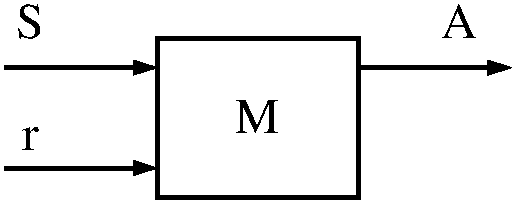
\includegraphics{media/page4diagram.pdf}}
\end{center}

assume a Markov decision process M which can be completely represented as a tuple \( M = \langle S, A, T, R, \pi, \tilde{T}, \tilde{R}\rangle \)\\

\begin{minipage}{5in}
\(S\) -- a set of states $s\in S$ which may be experienced by $M$\\
$A$ -- a set of actions $a\in A$ that may be executed\\
$T$ -- a true transitional probability, $T(s^{\prime}|a,s)$ expressing the probability of executing an action $a$ in state $s$ before ending up in later state $s^{\prime}$.\\
$R$ -- is a reward function which quantifies how desirable a transition $R(s'|a,s)$ is. $R: S\times S\rightarrow \mathbb{R}_{\geq 0}$\\
\textbf{[I changed $\mathbb{R}^{+}$ to $\mathbb{R}_{\geq 0}$ because the former is ambiguous with respect to whether or not 0 is included (online research suggests there is no accepted convention) while the latter is unambiguous.]}\\
$\pi$ -- is an action selection policy, ideally chosen to maximize expected reward, an optimal policy is denoted $\pi^*$. Typically
\begin{equation*}
\pi^*(s) = \argmax_{a}\sum_{s^\prime}\underbrace{R(s^\prime|a,s) T(s'|a,s)+\gamma V(s^\prime)}_{\text{expected reward}}
\end{equation*}
\end{minipage}

\section*{encoding}

To encode the expected reward over all states, typically $Q$-values are kept: \( Q(s,a) \sim \sum R(s^\prime|a,s)T(s^\prime|a,s)+\gamma V(s^\prime) \) and \( Q_{t+1}(s,a) \leftarrow Q_t(s,a)+\alpha \left( R(s^\prime|a,s)-Q_t(s,a)+\gamma\argmax)_{a^\prime} Q(s^\prime,a^\prime) \right) \).

In this paper we rely on a method of extracting dynamic $Q$-values from an encoded transition and reward function $( \tilde{T}, \tilde{R} )$. The motivation for this encoding is that it allows mapping the transition function into multiple spaces, and allows the reward function to be altered. The significance of this finding is covered in \textbf{???} Price wash \textbf{???}.

 


\newpage

\section*{page 5}

\section{Reconfiguration}

Reconfiguring \textbf{???} Process $M$ allows some intractable MDPs to be rendered tractable. 
As an example, a three dimensional foraging experiment with three thousand positions on the $x$, $y$, and $z$
axes respectively will consume over three billion memory locations and may be impossible to explore. If this system is
broken into three sub problems, each targets a special axis, the only nine thousand memory locations need be consumed. This decreases memory requirements by an exponential factor.

This paper presents a method of decomposition that, when followed, introduces no degeneration of the found policy $\pi^{*}(s,a)$.
The summary of these conditions is presented.

\section*{Summary of Requirements}

\section*{Introduction to approach}

\begin{equation*}
d^{M_i,M_k}_{M} = M \longrightarrow \left\{    M_i, M_k \middle|
\begin{array}{l}
S_i\times(S_k/s_i)=S, S_k\times(S_i/s_k)=S\\
A=A_i \cup A_k\\
\tilde{T}\sim d^{-1}(d(\tilde{T})),d(\tilde{T})=\tilde{T}_i, \tilde{T}_k\\
\tilde{R}\sim d^{-1}(d(\tilde{R})), d(\tilde{R})=\tilde{R}_i,\tilde{R}_k
\end{array}
 \right\}
\end{equation*}
where $d$, $d$ represent belief mapping functions that decompose and recompose mapping functions. This allows   \textbf{???} to be mapped as new spaces and observes are encountered. The decomposition process breaks one MDP into a parent and child:\\

\textbf{[This diagram hasn't been drawn yet because I'm prioritizing transcribing math and text over doing the diagrams.]}


\newpage

\section*{page 7}

The system can be broken into the following MDP definitions

\underline{$M_i$ -- Parent}

$S_i$ -- a collection of states, $s_i\in S_i$\\
$A_i$ -- a collection of actions, $a_i \in A_i$\\

$P(s^\prime_i|s_i, a_i)$ is observed directly\\

$R_t\left({}^{s^\prime_i}_{a^\prime_k}|{}_{a_i},{}^{s_i}_{a_k}\right)=R_t\left({}^{s^\prime_i}_{s^\prime_k},{}^{a_i}_{a_k},{}^{s_i}_{s_k}\right)$

\underline{$M_k$ -- child}

$S^\prime_i$ -- all child states, $s_k\in S_k$\\
$a_k\in A_k$\\
$P(s^\prime_k|s_k,a_k)$\\
$R_t(s^\prime_k,a_k,s_k)=R_t\left({}^{s_i}_{s^\prime_k},{}^{a_i}_{a_k},{}^{s_i}_{s_k}\right)$

\newpage

\section*{page 8}

\underline{Definitions}\\

\underline{$M$}\quad
\begin{minipage}[t]{5in}
$S=(S_i/S_k)\times(S_k/S_i)$\\
$A=A_i\cup A_k$\\
$T=P(S\times A\times S)$\\
$R= \text{real, positive, convergent stochastic as $t\to\infty$}$\\
$R(s^\prime,a,s) =R\left( 
\begin{array}{c} s^\prime_i \\ s^\prime_k \end{array},
\begin{array}{c} a_i \\ a_k \end{array},
\begin{array}{c} s_i \\ s_k \end{array}
\right)$
\end{minipage}\\

\underline{Parent MDP}\\


\underline{$M_i$}\quad
\begin{minipage}[t]{5in}
$S_i $, $s_i\in S_i$\\
$a_i\in A_i$\\
$P\left(
\begin{array}{c} s^\prime_i \\ a^\prime_k \end{array}
\middle|
\begin{array}{c}a_i \\ a_k \end{array},
\begin{array}{c} s_i \\ s_k \end{array}
\right)$\\
$R_t\left( 
\begin{array}{c} s^\prime_i \\ a^\prime_k \end{array},
\begin{array}{c} a_i \\ \end{array},
\begin{array}{c} s_i \\ a_k \end{array}
\right)
=
R_t\left( 
\begin{array}{c} s^\prime_i \\ s^\prime_k \end{array},
\begin{array}{c} a_i \\ a_k\end{array},
\begin{array}{c} s_i \\ s_k \end{array}
\right)
\quad\text{
s.t.}\ s_k, s^\prime_k\ \text{are not directly observable}$\\
$a_k=\pi_k(s_k)$\\
$a^\prime_k=\pi_k(s^\prime_k)$
\end{minipage}\\

$\ast \rule[3pt]{3cm}{0.1pt}$\fbox{assume $s_k$, $s^\prime_k$ chosen s.t.\ as $t\to\infty\quad E[R_{t+1}()]\geq E[R_t(\cdot)]$}\\


\underline{Child MDP}\\

\underline{$M_k$}\quad
\begin{minipage}[t]{5in}
$S_k, s_k\in S_k$\\
$a_k\in A_k$\\
$P(s^\prime_k|s_k,a_k)$\\
$R_t(s^\prime_k, a_k, s_k)=R_t\left(
\begin{array}{c}s^\prime_i \\ s^\prime_k \end{array},
\begin{array}{c}a_i \\ a_k\end{array},
\begin{array}{c}s_i \\ s_k \end{array}
\right)\quad\text{s.t.}\ s_i,s^\prime_i\ \text{are chosen by another process}$
$a_i=\pi_i(s_i)$\\
$\ast\qquad$ time monotonicity assumed.
\end{minipage}\\

\newpage

\section{Mapping function}
\label{sec:mapping}

After defining Parent and Child MDPs, it is important to note how to map information from a centralized MDP onto a parent-child pair: (equation $d^{M_j, M_k}_{M_i}$) $d^{M_j, M_k}_{M_i}$ . To expedite convergence and computational proofs that follow, a mapping function $d^{M_j, M_k}_{M_i}$ is assume to have Basic Requirements (Sec.~\ref{sec:basicrequirements}). Afterward the process is explained (Sec.~\ref{sec:mappingprocess}).

\subsection{Basic mapping requirements}
\label{sec:basicrequirements}

$S_i$, $S_j$, $S_k$: \quad $S_j \times (S_k/S_j)  \supseteq S_i$,\quad $S_k \times (S_j/S_k) \supseteq S_i$\\

Sets $S_k$ and $S_j$ must be able to be combined to make the original set.\\

$A_i$, $A_j$, $A_k$: \quad $A_i \subseteq A_j\cup A_k$\\

Also, action sets must combine to recover the original action set.\\

$T_i$, $R_i$ $\sim$ unknown/unknowable, stable decomposition\\

The true transition and reward functions may remain unknown.\\

more$\longrightarrow$
\fbox{\pbox[b]{\textwidth}{\qquad\qquad assumed\\
$\ast$ important to select so that $\tilde{T}_i$ \& $\tilde{T}_k$ seem independent}}\\

\subsection{Mapping process}
\label{sec:mappingprocess}

Transition mapping:\\

$\exists f_1:\tilde{T}_i\to \tilde{T}_j, \tilde{T}_k$,\ invertible; $\tilde{T}_i = f_1\left(f^{-1}\left(\tilde{T}_i\right)\right)$\\
$\exists f_2:\tilde{R}_i\to \tilde{R}_j, \tilde{R}_k$,\ invertible; $\tilde{R}_i = f_2\left(f_2^{-1}\left(\tilde{R}_i\right)\right)$\\

\underline{Transition function mapping: knowing $s_x\in S_x$, $s_y\in S_y$} (1 way)\\

Goal $\exists f:P(S_x|A,S_x)\leftarrow P(S|A,S)$\\
knowing $P(S_x \times S_y | A_x \cup A_y, S_x \times S_y)=P(S|A,S)$

Clearly: 
\begin{equation*}
P(s^\prime_x|s_x,a_x) = \sum_{s_y^\prime}\sum_{a_y}\sum_{s_y} P\left( s_x^\prime,s_y^\prime|s_x,s_y,a_x,a_y\right)P\left(a_y|S_y \right)P\left( s_y \right)
\end{equation*}

\begin{equation*}
\therefore\quad\tilde{T}\left( s^\prime_x \middle| s_x, a_x \right) = \sum_{s^\prime_y} \sum_{a_y} \sum_{s_y} \tilde{T}\left( s^\prime \middle| a, s  \right) \underbrace{\tilde{\pi}\left( a_y \middle| s_y \right)}_{\text{require policy mapping}}P(s_y)
\end{equation*}

Action mapping:\\

\underline{Action mapping} (1 way)\\

Next, we can consider an action mapping where actions from $A$ can be randomly assigned to $A_x$, $A_y$: $A_x \leftarrow \left\{ a\in A^\prime \middle| A^\prime \subseteq A \right \}$, $A_x, A_y\subseteq A$, $A_x \cup A_y = A$, $A_x \neq \{ \null \}$, $A_y \neq	 \{ \null \}$.\\

\underline{General approach}: \underline{High reward for \textbf{???}ve states}\\

Given $\tau \in \mathbb{R}$, $\pi(a|s)$, $\tilde{Q}(a,s)$ then 
\begin{equation*}
A_x \leftarrow A_x \cup \left\{ a  \middle| \underbrace{ \pi(a|s) \tilde{Q}(a,s) > \tau }_{\text{condition}} \right\}
\end{equation*}
or, more usefully/generally
\begin{equation*}
A_x \leftarrow A_x \cup \left\{ a \middle| \underbrace{ \left( \pi (a \middle|  S_s^{R^\prime} \right) \tilde{Q}(a,S^{*\prime}) > \tau }_{\text{condition}} \right\}
\end{equation*}
where
\begin{equation*}
S_s^{*\prime}=\left\{ S^\prime \middle| S/s_s^* \neq S\right\} \qquad\text{(see p. ???)}
\end{equation*}

Condition options:
\begin{equation*}
\ast \text{reformulation over set }S\text{\ vs.\ }s\in S\qquad 
\left\{ 
\begin{array}{l}
\text{a)\ }\pi(a|s)\tilde{Q}(a,s)>\tau \qquad \cdots \quad \text{High reward} \\
\text{b)\ }\pi(a|s)\tilde{Q}(a,s)>\tau,\quad\pi(a|s)>0\qquad \cdots \quad \text{small reward}
\end{array}
\right.
\end{equation*}



(Network approach)\\ 




\newpage

\section{Worst Case Performance}
\label{sec:worstcase}

\subsection{Computational Complexity}
 \label{sec:complexity}

\underline{Total Mapping}\\

 
$\ast\ A_R = \left\{ \begin{array}{l} \text{State 1, State 2, Action 1, Action 2} \\ \text{merge, time up, time down} \end{array} \right\}$\\

Given\ 
\begin{minipage}[t]{0.7\textwidth}
$S\in\mathbb{R}^{n}$, define dimensions $\{i_s\}_{i_s=1}^{n}$ \\
$A\in \mathbb{N}^{m}$, define dimensions $\{i_r\}_{i_r=1}^{m}$
\end{minipage}\\

Then, with an initial MDP $M=\langle S, A, T, R, \pi, M_R \rangle$, all possible ``sub mdps'' $M_1$, $M_2$, $M_3$, \ldots represent the family of MDPs which can be created from $M$, $\mathscr{P}(M)=\left\{M_x | S_x \subseteq S, A_x\subseteq A, R, \pi \text{\ from MDPs \textbf{???}}\right\}$ and each member $M_x$ is characterized by a language $J_{sx}\subseteq \left\{i_s\right\}_{i_s=1}^{n}$ or $J_{sy}\subseteq\left\{i_r\right\}_{i_r=1}^{m}$ where $J_{sx}\times J_{sy}$ defines a space $S_R$, for the reconfiguration MDP to explore, with actions from $A_R$.\\

\begin{equation*}
J \left| \begin{array}{l}\text{Reward is defined as average expected reward over an epoch $e$.} \\ \text{in terms of transition} \end{array} \right.
\end{equation*}\\

$\ast\ S_R = \mathscr{P}\left(\left\{i_s\right\}_{i_s=1}^{n}\right)\times\mathscr{P}\left(\left\{i_r\right\}_{i_r=1}^{m}\right)$
$\qquad\longleftarrow\ $ exponentional increase in space (stupid!)
\\

Problems\ 
\begin{minipage}[t]{0.5\textwidth}
1)\ exponential space consumption\\
2)\ how to handle chaining/nesting\\
3)\ how to structure action choice policy
\end{minipage}

\newpage

\section{Mapping as a process}

In this section it is described how, and when, the function $d^{M_j, M_k}_{M_i}$ is applied. In fact, instead of structing the application of $d^{M_j, M_k}_{M_i}$ as human chosen conditional statements, it is possible to consider when to ``split'' and ``merge'' and MDP $M_i$ into $M_j$, $M_k$ as a learning problem. This problem is expressed as the mapping problem, and modelled as a learning problem MDP-map ($M_{\text{map}}$):
\begin{equation*}
M^i_{\text{map}} = \left\langle S^{i}_{\text{map}}, A^{i}_{\text{map}}, T^{i}_{\text{map}}, R^{i}_{\text{map}} \right\rangle
\end{equation*}

\begin{equation*}
S_{\text{map}} = f\left( d\left( M_i, \mathscr{P}\left( M_j \right), P\left( M_k \right) \right) \right)\,,\quad\text{s.t.\ }
f: d^{M_j, M_k}_{M_i} \to \mathbb{R} 
\end{equation*}
where $d\left( M_i, M_j, M_k \right) = d^{M_j, M_k}_{M_i}$.\\

The state encodes all possible configurations for the MDP split:\\
\textbf{[FIGURE]}\\
\begin{align*}
A^{i}_{\text{map}} & = 
\text{a set of actions formed from the the decomposition and recomposition functions\: } \\
& \qquad \qquad
A_{\text{decomposition}} \cup \left\{ a_r \right\} \\
& \quad
\text{where\ }a_r \text{\ is a special recomposition function.}\\
T^{i}_{\text{map}} & = \left\{ 
\begin{array}{cl} 1\,, & \left( S = S_1 \text{\ and\ } a \neq a_r \right) \text{\ or\ } \left( S \neq S_1 \text{\ and\ } a = a_r \right)  \\ 0\,, & \text{otherwise} \end{array} 
\right. \\
R^{i}_{\text{map}} & = \sum_{e=\text{epoch}}R^{i}(e) \\
\end{align*}



Given $(S_{\textrm{map}}, A_{\textrm{map}}, T_{\textrm{map}}, R^{i}_{\textrm{map}}, \pi_{\textrm{map}})$, applied to $M=\langle S_x, A_x, \tilde{T}_x, R_x, \tilde{\pi}_x \rangle$, we may trivially define $M_y=\langle S_y, A_y, \tilde{T}_y, R_y, \pi_y \rangle$ in a method consistent with Bush, p.\ 74, with $M_x$ being the parent process and $M_y$ being the child.\\

a) for $R^{i}_{\textrm{map}}$, there are five versions $i\in\{1,\ldots,5\}$\\
b) Given $M_x$, $M_y$, a merge is also possible, so recovering $M$\\
c) we can perform temporal Sink actions on an MDP (Book I, p.\ 88)\\
${}\qquad\hookrightarrow$\ reduce resolution\\
${}\qquad\hookrightarrow$\ re-increase resolution\\

\underline{Actions}\\

$\therefore$ Seven ``actions'' can be performed on an MDP: $(M_R)$\\

$\qquad$\begin{minipage}[t]{0.9\textwidth}
\underline{State}\\

\begin{equation*}
\left\{R^i_{\textrm{map}}\right\}_{i=0}^{5}\cup \left\{\text{merge}\right\}\times\left\{\text{scale\ up}^{i}\right\}_{i=0}^{5}\cup\left\{\text{normal}\right\}\cup\left\{\varnothing\right\}
\end{equation*}\\

\underline{Reward}\\

\begin{equation*}
R(s^\prime,a,s)=\sum_{l\in e}R(l)\qquad\text{reward during a trajectory}
\end{equation*}
$e=\text{epoch}$\\

\underline{Transition}\\

-easy to explain in MS Word
\begin{equation*}
T=\left\{
\begin{array}{l}
1\ \text{-- allow \textbf{???}}\\
0\ \text{-- otherwise}
\end{array}
\right.
\end{equation*}
\end{minipage}



\newpage



\underline{Reward function mapping (5 way)}\\

knowing $R\left(\{s_x, s_y\}|a, \{s^\prime_x,s^\prime_y\}\right)=R(s|a,s)$\\




\underline{Mapping Policy} (1 way)\\

finding: $f\tilde{\pi}(s)\to f\tilde{\pi}(s_y)$\\

\begin{equation*}
\tilde{\pi}(a_y|s_y) \leftarrow \sum_{s_x}\sum_{a_x}\tilde{\pi}\left( \{ a_x, a_y \} \middle|  \{ s_x, s_y \} \right)P(s_x) 
\end{equation*}

\newpage

\section*{page 14}

\underline{Mapping Policy} (1 way)\\

finding: $f\tilde{\pi}(s)\to f\tilde{\pi}(s_y)$\\

\begin{equation*}
\tilde{\pi}(a_y|s_y) \leftarrow \sum_{s_x}\sum_{a_x}\tilde{\pi}\left( \{ a_x, a_y \} \middle|  \{ s_x, s_y \} \right)P(s_x) 
\end{equation*}

\newpage

\section*{page 15}

\underline{Action mapping} (1 way)\\

Next, we can consider an action mapping where actions from $A$ can be randomly assigned to $A_x$, $A_y$: $A_x \leftarrow \left\{ a\in A^\prime \middle| A^\prime \subseteq A \right \}$, $A_x, A_y\subseteq A$, $A_x \cup A_y = A$, $A_x \neq \{ \null \}$, $A_y \neq	 \{ \null \}$.\\

\underline{General approach}: \underline{High reward for \textbf{???}ve states}\\

Given $\tau \in \mathbb{R}$, $\pi(a|s)$, $\tilde{Q}(a,s)$ then 
\begin{equation*}
A_x \leftarrow A_x \cup \left\{ a  \middle| \underbrace{ \pi(a|s) \tilde{Q}(a,s) > \tau }_{\text{condition}} \right\}
\end{equation*}
or, more usefully/generally
\begin{equation*}
A_x \leftarrow A_x \cup \left\{ a \middle| \underbrace{ \left( \pi (a \middle|  S_s^{R^\prime} \right) \tilde{Q}(a,S^{*\prime}) > \tau }_{\text{condition}} \right\}
\end{equation*}
where
\begin{equation*}
S_s^{*\prime}=\left\{ S^\prime \middle| S/s_s^* \neq S\right\} \qquad\text{(see p. 12)}
\end{equation*}

Condition options:
\begin{equation*}
\ast \text{reformulation over set }S\text{\ vs.\ }s\in S\qquad 
\left\{ 
\begin{array}{l}
\text{a)\ }\pi(a|s)\tilde{Q}(a,s)>\tau \qquad \cdots \quad \text{High reward} \\
\text{b)\ }\pi(a|s)\tilde{Q}(a,s)>\tau,\quad\pi(a|s)>0\qquad \cdots \quad \text{small reward}
\end{array}
\right.
\end{equation*}

\underline{Transition function mapping: knowing $s_x\in S_x$, $s_y\in S_y$} (1 way)\\

Goal $\exists f:P(S_x|A,S_x)\leftarrow P(S_x|A,S)$\\
knowing $P(S_x \times S_y | A_x \cup A_y, S_x \times S_y)=P(S|A,S)$

Clearly: 
\begin{equation*}
P(s^\prime_x|s_x,a_x) = \sum_{s_y^\prime}\sum_{a_y}\sum_{s_y} P\left( s_x^\prime,s_y^\prime|s_x,s_y,a_x,a_y\right)P\left(a_y|S_y \right)P\left( s_y \right)
\end{equation*}

\begin{equation*}
\therefore\quad\tilde{T}\left( s^\prime_x \middle| s_x, a_x \right) = \sum_{s^\prime_y} \sum_{a_y} \sum_{s_y} \tilde{T}\left( s^\prime \middle| a, s  \right) \underbrace{\tilde{\pi}\left( a_y \middle| s_y \right)}_{\text{require policy mapping}}P(s_y)
\end{equation*}


\newpage

\subsection{}

\subsubsection{Proof of Decomposition Correctness (Process 1)}

The following section demonstrates\\

\underline{MDP Policy Decomposition}\\

First, it is true that the optimal policy $\pi^\ast(s)$ for a centralized MDP will arise from maximizing the expected reward.

\begin{equation*}
\pi^\ast(s) = \argmax_{a} \sum_{s^\prime} R(s,a,s^\prime) P(s^\prime |s, a) + \gamma V(s^\prime)
\end{equation*}

It is now shown that a set of MDPs ($M_i$, $M_k$) can be observed to create an optimal policy $\exists f s.t.\ f\left( \pi^\ast_i, \pi^\ast_k \right) \sim \pi^\ast$.

Given $\pi^\ast_i(S_i, A_k)$, $\pi^\ast_k(S_k)$

\begin{equation*}
1.\quad \pi^\ast(s_i,s_k) = \argmax_{a_i, a_k} \sum_{s^\prime_i} \sum_{s^\prime_k} R\left( (s_i,s_k),(a_i,a_k),(s^\prime_i,s^\prime_k)\right) P\left( (s^\prime_i, s^\prime_k) \middle| (s_i, s_k), (a_i, a_k)  \right)
\end{equation*}

\textasteriskcentered \quad \underline{Lemma 1 -- augmentation with $a_k$}\quad where $a^\prime_k=\pi^\ast(s^\prime_k)$

\begin{equation*}
2.\quad\pi^\ast(s_i, s_k) = \argmax_{a_i, a_k} \sum_{s^\prime_i} \sum_{s^\prime_k} R\left((s_i, s_k, a_k), (a_i,a_k),(s^\prime_i,s^\prime_k,a^\prime_k) \right) P\left( (s^\prime_i, s^\prime_k, a^\prime_k) \middle| (s_i, s_k), (a_i,a_k) \right) 
\end{equation*}

\textasteriskcentered \quad \underline{Lemma 2 -- Simplification}\\

$\overbrace{\ast\quad\text{assume} \quad \argmax_{a_i,a_k} \equiv \argmax_{a_i} \argmax_{a_k}}^{\text{separability}}$\\

 \begin{equation*}
3.\quad\pi^\ast(s_i, s_k) = \argmax_{a_i, a_k} \sum_{s^\prime_i}  R\left((s_i, a_k), (a_i,a_k),(s^\prime_i, a^\prime_k) \right) P\left( s^\prime_i, a^\prime_k \middle| (a_i,a_k),  (s_i, s_k) \right) 
\end{equation*}

\underline{Lemma 3}\\

\textasteriskcentered \quad separation of $a_k$, and $a_k \leftarrow \pi^{\ast}_k(s_k)$

 \begin{equation*}
4.\quad\pi^\ast(s_i, s_k) =\left( \argmax_{a_i} \sum_{s^\prime_i}  R\left((s_i, a_k), a_i,(s^\prime_i, a^\prime_k) \right) P\left( s^\prime_i, a^\prime_k \middle| a_i,  (s_i, s_k) \right) \right)
\end{equation*}

\textasteriskcentered \quad \underline{Lemma 4}\\

\begin{equation*}
a_i = \pi^\ast_i(s_i) \longrightarrow^{\cup} \left( \argmax_{a_k} \sum_{s^\prime_k}  R\left(s_k, a_k, s^\prime_k, a^\prime_k \right) P\left( s^\prime_k \middle| a_k, s_k \right) \right)
\end{equation*}

\begin{center}
\fbox{
\begin{minipage}{5cm}
\begin{equation*}
5.\quad\pi^\ast(s_i, s_k) = \pi^\ast_i(s_i,a_k)\cup \pi^\ast(s_k)
\end{equation*}
\end{minipage}
}
\end{center}

Thus, given $\pi^\ast_i$ and $\pi^{i}_{k}$, it is possible to infer $\pi^\ast \left( s_i, s_k \right)$.\\

We now prove lemmas involved.\\

Lemma 1:\\
\vspace*{4cm}

Lemma 2:\\
\vspace*{4cm}

Lemma 3:\\
\vspace*{4cm}

Lemma 4:\\
\vspace*{4cm}

\newpage

\section*{page 15.2}

\underline{MDP Policy Decomposition}\\

\begin{equation*}
\pi^\ast(s) = \argmax_{a} \sum_{s^\prime} R(s, a, s^\prime) P(s^\prime | s, a) +\gamma V(s)
\end{equation*}

Given $\pi^\ast_i(S_i,A_k)$, $\pi^\ast(S_k)$\\

\begin{equation*}
1.\quad \pi^\ast(s_i,s_k) = \argmax_{a_i, a_k} \sum_{s^\prime_i} \sum_{s^\prime_k} R\left( (s_i,s_k),(a_i,a_k),(s^\prime_i,s^\prime_k)\right) P\left( (s^\prime_i, s^\prime_k) \middle| (s_i, s_k), (a_i, a_k)  \right)
\end{equation*}\\

Note:\qquad
\begin{minipage}[t]{10cm}
$R\left( (s_i,s_k,a_k),(a_i,a_k),(s^\prime_i,s^\prime_k) \right) \leftarrow R\left((s_i,s_k),(a_i,a_k),(s^\prime_i,s^\prime_k)\right)$\\
$R\left( (s_i,s_k,a_k),(a_i,a_k),(s^\prime_i,s^\prime_k,a^\prime_k) \right) \leftarrow R\left((s_i,s_k),(a_i,a_k),(s^\prime_i,s^\prime_k)\right)$
\end{minipage}\\


\textasteriskcentered assume separability $\longrightarrow$\\
\begin{align*}
2.\quad \pi^\ast(s_i,s_k) & = \argmax_{a_i} \argmax_{a_k} \sum_{s^\prime_i} \sum_{s^\prime_k} R\left( ( s_i, s_k, a_k ), ( a_i, a_k ), ( s^\prime_i, s^\prime_k, a^\prime_k )\right) P\left( ( s^\prime_i, s^\prime_k, a^\prime_k ) \middle| \cdot \right) \\
& = \argmax_{a_i} \sum_{s^\prime_i} \sum_{s^\prime_k} R\left(  ( s_i, s_k, a_k ),\begin{array}{c} a_i \\ a_k \end{array}
\middle| 
\begin{array}{c} s^\prime_i \\ s^\prime_k \\ a^\prime_k \end{array}
\right)
P\left( 
\begin{array}{c} s^\prime_i \\ s^\prime_k \\ a^\prime_k \end{array}
\middle | \begin{array}{c} a_i \\ a_k \end{array},
\begin{array}{c} s_i \\ s_k \\ a_k \end{array}
\right) \\
& \qquad \qquad \qquad
\cup
\argmax_{a_k}
 \sum_{s^\prime_k} R\left(  \begin{array}{c} s_i \\ s_k \\ a_k \end{array},\begin{array}{c} a_i \\ a_k \end{array}
\middle| 
\begin{array}{c} s^\prime_i \\ s^\prime_k \\ a^\prime_k \end{array}
\right)
P\left( 
\begin{array}{c} s^\prime_i \\ s^\prime_k \\ a^\prime_k \end{array}
\middle | \begin{array}{c} a_i \\ a_k \end{array},
\begin{array}{c} s_i \\ s_k \\ a_k \end{array}
\right)
\end{align*}\\

\begin{align*}
\ast\qquad \text{let\ }a_k^\ast & = \argmax_{a_k}\sum_{s^\prime_k}  R\left(  \begin{array}{c} s_i \\ s_k \\ a_k \end{array},\begin{array}{c} a_i \\ a_k \end{array}
\middle| 
\begin{array}{c} s^\prime_i \\ s^\prime_k \\ a^\prime_k \end{array}
\right)
P\left( 
\begin{array}{c} s^\prime_i \\ s_k \\ a_k \end{array}
\middle | \begin{array}{c} a_i \\ a_k \end{array},
\begin{array}{c} s_i \\ s_k \\ a_k \end{array}
\right)\\
& \qquad\text{s.\ t.\ }s_i,s^\prime_i\leftarrow\pi^\ast_i( \\
&\qquad\quad a^\ast_i = \pi^\ast_i(s)
\end{align*}

\begin{align*}
3.\qquad &= \argmax_{a_i}\sum_{s^\prime_i}
 R\left(  \begin{array}{c} s_i \\ a_k \end{array},
\begin{array}{c} a_k \\ a^\ast_k \end{array},
\begin{array}{c} s^\prime_i \\  a^\prime_k \end{array}
\right)
P\left( 
\begin{array}{c} s^\prime_i \\ a^\prime_k \end{array}
\middle | \begin{array}{c} a_i \\ a^\ast_k \end{array},
\begin{array}{c} s_i \\ a_k \end{array}
\right)
\cup
\pi^\ast_k(s_k)=a_k \\
& = \pi^\ast_i\left( s_i \middle| \pi_k^\ast \right) \cup \pi^\ast_k(s_k)
\end{align*}

\newpage

\section*{page 16}

\begin{center}
Parent Policy Convergence
\end{center}

\underline{For the Parent MDP $M_k$}\\

--from definition $E\left[ R_t \left( s^\prime_k \middle| a_k, s_k \right) \right] \ge E\left[ R_{t+1}\left( s^\prime_k \middle| a_k, s_k  \right) \right]$\\
\begin{align*}
R_t\left( s^\prime_i \middle| a^\prime_i, s^\prime_i \right) & = R\left( \begin{array}{c} s^\prime_i \\ s^\prime_k \end{array} \middle| 
\begin{array}{c}a_i \\ a_k \end{array}, \begin{array}{c} s_i \\ s_k \end{array} \right)\\
& \text{i.}\qquad a_k = \pi_k( s_k )\\
& \qquad\quad ( s^\prime_k, s_k ) \text{\ result from\ }a_i\text{\ s.t.\ }\\
&\text{ii.}\qquad s^\prime_k \sim T( S_k | \pi_i( s_k ), s_k )\\
&\text{iii.}\qquad s_k \sim T( S_k | \pi_i( s^\ast_k ), s^\ast_k )
\end{align*}

A)\\
\boxed{$\textasteriskcentered$} -- $\pi_k(\cdot)$ is effective: $E\left[ R\left( \begin{array}{c} s^\prime_i \\ s^\prime_k \end{array} \middle| \begin{array}{c} a_i \\ a^\ast_k \end{array}, \begin{array}{c} s_i \\ s_k \end{array} \right) \right] 
\ge E\left[ R\left( \begin{array}{c} s^\prime_i \\ s^\prime_k \end{array} \middle| \begin{array}{c} A_i \\ A_k \end{array}, \begin{array}{c} s_i \\ s_k \end{array} \right) \right]$\\
\qquad\qquad$\exists a_i, a^\ast_k\leftarrow\pi_k(s_k)$\\

B)\\
\boxed{$\textasteriskcentered$} -- $\pi_k(\cdot)$ is convergent:
\begin{equation*}
E\left[ R_{t+1}\left( \cdot \middle| \pi_{\substack{k\\t+1}},\cdot\right)\right] \ge E\left[ R_{t+1}\left( \cdot \middle| \pi_{\substack{k\\t+1}},\cdot\right)\right]
\end{equation*}

 assume some policy $\pi_k(\cdot)$ is both effective and convergent, then:\\
$\textcircled{\text{A}}+\textcircled{\text{B}}\rightarrow\textcircled{\text{C}}$\\

C)\\

\begin{equation*}
\boxed{\ast}\qquad \lim_{t\rightarrow\infty} R_t\left( s^\prime_i \middle| a_i, s_i \right) \sim R_{t+1}\left( s^\prime_i \middle| a_i, s_i \right)
\end{equation*}

E) Show other typical convergence \textbf{???},\\

Done\\

\underline{For the child}\\

\boxed{$\textasteriskcentered$}$\qquad\qquad$ \underline{trivial}




\newpage

\section*{page 16.1}

\begin{enumerate}[label=\protect\textcircled{\arabic*}]
\setcounter{enumi}{2}
\item Tractability: it is not possible to map infinite state spaces in practice, so it is advantageous to set up $f_Q$ on a 
subspace \begin{align*}
\mathfrak{Z} & = S \times A \times S \\
\text{s.t.:}\qquad & f_Q: \tilde{T}_t( \mathfrak{Z} ) \times \tilde{R}_t ( \mathfrak{Z} ) \rightarrow Q_t( \mathfrak{Z} )\qquad\qquad \leftarrow\text{(sloppy)}
\end{align*}
which more or less can be directly incorporated into $Q_t$:
\begin{equation*}
f_m: Q_{t+1}( S \times A ) \times Q_t(\mathfrak{Z}) \rightarrow Q_t(S\times A)
\end{equation*}
We also need to keep $\tilde{T}$ and $\tilde{R}_t$ updated and can employ \textbf{???} regression instances to do this
\begin{align*}
f_T: & \tilde{T}_{t-1}(\mathfrak{Z})\times\{s,a,s^\prime\}\rightarrow \tilde{T}_t(\mathfrak{Z}) \\
f_R: & \tilde{R}_{t-1}( \mathfrak{Z} ) \times \left\{  R( s^\prime | a, s ) \right\} \rightarrow \tilde{R}_t( \mathfrak{Z} )
\end{align*}
\hrule
{\ }\\

\item Implementation: I use instances of stochastic gradient descent to regress \fbox{$f_T$} and \fbox{$f_R$}
\begin{equation*}
\tilde{T}_t(s^\prime | a, s ) \leftarrow f_T(s,a,s^\prime,T_{t-1}) = \tilde{T}_{t-1}(s^\prime|a,s)+\alpha_T\left(\frac{f_r(s,a,s^\prime)}{f_r(s,a)}-T_{t-1}(s^\prime|a,s)\right)
\end{equation*}
\begin{equation*}
\tilde{R}_t \leftarrow\text{\ user defined (in this case), and is readily ``pulled''}
\end{equation*}
where $f_r(s,a,s^\prime)$ and $f_r(s,a)$ reflect visitation frequencies.\\

$f_Q$ is more difficult, and can be broken into exact solutions and approximate solutions
\begin{equation*}
Q_t(s,a) \leftarrow f_Q^{\text{exact}}\left( \mathfrak{Z}, \tilde{T}_t, \tilde{R}_t \right) = \sum_{s^\prime \in \mathfrak{Z}} \tilde{T}(s^\prime|s,a) \tilde{R}(s^\prime|s,a) +\gamma V(s^\prime)
\end{equation*}
where $V(s)\approx \argmax_{a} Q_{t-1}(s,a)$, where $\mathfrak{Z}=S \times A$ yields the more accurate and intractable model, it may be desired to focus on estimation, $f_a^{\text{est}}$.

\end{enumerate}

\newpage

\section*{page 17}

On The Generalization and reuse of transitional knowledge \#2\\

\hrule
{\ }\\
\begin{enumerate}[label=\protect\circled{\arabic*}]

\item Setting the state, taking a general FOMDP given usual expections (stably stochastic etc.) $m=\langle S,A,T,R \rangle$ want to find $\pi^{\ast}:\left\{ S \times A \right\} \cup Q(S,A) \rightarrow A$ s.\ t.\ for some value function $V(s)$, $\pi^{\ast}(s) = \argmax_{a} \sum_{s^\prime} T \left( s^\prime \middle| a, s \right) R\left( s^\prime \middle| a, s \right) + \gamma V(s^\prime)$\\

Traditionally, convergence can be found directly, using stochastic gradient descent
\begin{equation*}
Q_{t+1}(s,a) = Q_t(s,a) +\alpha\left( R(s^\prime|s,a) -Q_t(s,a) + \gamma \argmax_{a} \left( Q_t(s^\prime, a^\ast )\right)\right)
\end{equation*}
which is limited because as $Q(S,A)$ converges, it becomes difficult to adjust to changes in $R(S,A,S)$.
{\ }\\
\hrule
{\ }\\

\item Optimization objectives change, meaning the basis of $Q(S,A)$ is typically malleable in real-life scenarios. In this paper we present a method for separating transitional models and reward models.

We hold reward and transitional functioning separate as $\tilde{T}$ and $\tilde{R}$; and attempt to regress to true values s.\ t.\ $\tilde{T}\approx T$ and $\tilde{R} \approx R$. We then develop a $Q_{\text{map}}$ function $f_Q$ to \textbf{???} $Q(S,A)$ space as needed:
\begin{equation*}
f_Q:\tilde{T}\left( S \times A \times S \right) \times \tilde{R}\left( S \times A \times S \right) \rightarrow Q_t\left( S ,A \right)
\end{equation*}
\end{enumerate}

\newpage

\section*{page 18}

MDP: Linearization of Reward/Optimal Policy\\

$P_a$ -- $P_a(i,j)$ represents $T(s_i, a, s_j)$ $\qquad$ $S$-- all states\\
$\gamma$ -- decay factor $\qquad(0,1)$\\
$\pi$ -- policy \\
$V^\pi(s)$ -- typical value function\\
$\mathbf{V}^\pi$ -- vector of all values $\left\{ V^\pi(s_1),\ldots,V^\pi(s_n)\right\}$\\
$\prec$ and $\preceq$ denote strict and non-strict vectoral inequality.\\
$\mathbf{R}$ -- vector of reward (like $\mathbf{V}^\pi(s)$)\\

for optimal reward:
\begin{equation*}
\left( P_{a_i} - P_a \right) (I-\gamma P_{a_i})^{-1} \mathbf{R} \succeq 0\qquad\qquad\Leftrightarrow
\end{equation*}

Proof (cool as fuck):
\begin{equation*}
a_1 \equiv \pi(s) \in \argmax_{a\in A} \sum_{s^\prime} P_{s_a}(s^\prime)V^\pi(s^\prime) \quad\forall s \in S
\end{equation*}
\begin{align*}
\sum_{s^\prime}P_{s_{a_1}} & \geq \sum_{s^\prime}P_{s_a}(s^\prime)V^\pi(s^\prime) \quad \forall s \in S, a \in A \\
& \qquad \vdots \qquad \begin{array}{c} \rotatebox{90}{$\Rsh$} \\ \rotatebox{90}{$\Lsh$}  \end{array}  a_1 \text{\ is Pareto efficient (!)} \\
P_{a_1} \mathbf{V}^\pi & \succeq P_a V^\pi \quad \forall a\in A \backslash a_1\qquad \text{(non-strict improvement)}\\
& \qquad \vdots \\
P_{a_1}(I - \gamma P_{a_1})^{-1} \mathbf{R} &  \succeq P_a(I-\gamma P_{a_1})^{-1} \mathbf{R} \quad \forall a \in A\backslash a_1 
\end{align*}
The hard part to verify: $\mathbf{V}^\pi = (I-\gamma P_{a_1})\mathbf{R}$






\newpage

\section*{page 19}

\underline{Transitional Learning Continued}\\

\renewcommand{\labelitemi}{--}
\begin{itemize}
\item $\{s,s^\prime,w\}$ can be controlled to both represent the state space and accurately represent $P+(s^\prime|s^\prime,a)$\\
\item $A+h$, $B+h$ and $\gamma$ can be controlled to speed the algorithm $R_\gamma$\\
\item Q-learning can still be used, if calculation of $\bar{R}_\gamma$ is too ``slow''.\\
\item the reward function $R(s,a,s^\prime)$ can be redefined at an instant to allow immediate re-calculation of a policy $\bar{R}_\gamma(s,a)$.
\end{itemize}
{\ }\\
Possible experiments:\begin{minipage}[t]{\linegoal}
\begin{itemize}
\item show speed of convergence is greater, due to the ``storing'' of the transitional model across all actions\\
\item show that the generalized learning allows for redefinition of the reward function.
\end{itemize}
\end{minipage} 
\renewcommand{\labelitemi}{$\bullet$}

\newpage

\section*{page 20}

Policy\\
\underline{Convergence of ``Bad MDP''}\\

Question, given $\pi_i^\ast$, is it possible to find 
\begin{equation*}
f: \pi^\ast_j, \pi^\ast_k \rightarrow \pi^*_i
\end{equation*}
\begin{equation*}
f(\pi_j(s))
\end{equation*}
\begin{enumerate}[label=\alph*)]
\item suppose $f\left(\pi_j\left(s,\pi_k(s)\right)\right)=\pi_j\left( s,\pi_k(s)\right)\cup\pi_k(s)$\\
\item $S_k$,$S_j$ -- assume a subspace that is independent of effect by $A$, $S_j\in S_i$\\
$A_k$, $A_j$ -- assume a subset of $A_j$\\
$T_k$, $T_j$ -- assume $T(s_i,a,s^\prime_j)=0\quad\forall(s_i,a_j,s_j)\in S_j\times A_j \times S_j$\\
$R_k$, $R_j$ -- assume $R(s_i,a,s _j)$\\
In this case, $A_j$ \underline{must} effect $T(s_k,a_k,s^\prime_k)$ and $A_k$ \underline{must} \underline{effect} $T(s_j,a_j,s^\prime_j)$\\
\underline{effect how:}\\

\begin{minipage}{0.5\textwidth}
\begin{equation*}
\exists a_j, a_k \sum_{s^\prime_j\neq s_j}T\left( s^\prime_j \middle| \begin{array}{c} a_j \\ a_k \end{array}, s_j \right) > 0
\end{equation*}
\end{minipage}
\begin{minipage}{0.5\textwidth}
\fbox{\textasteriskcentered(Derive this conclusion from $T(s_i,a_i,s_i)$)\textasteriskcentered}
\end{minipage}\\
\item $M_j$, $M_k$ execute \underline{concurrently}, meaning at each time $t$ $\exists(a_j,a_k)\in A_i$, chosen by $a_j\sim \pi_j(s_j,a_k)\qquad a_k\sim\pi_k(s_k)$
\end{enumerate}

\newpage

\section*{page 21}

\underline{child convergence} assume during concurrent learning\\

\begin{itemize}
\item $R_t$ must be time-monotonic and convergent stochastic.\\
\item Evaluate selection of $s^\prime_i$ and $s_i$, assuming worst case: $a_k$ has no impact on $s^\prime_k$, $s_k$ and only an impact on $s_i$ and $s^\prime_i$\\
\begin{center}
\scalebox{0.5}{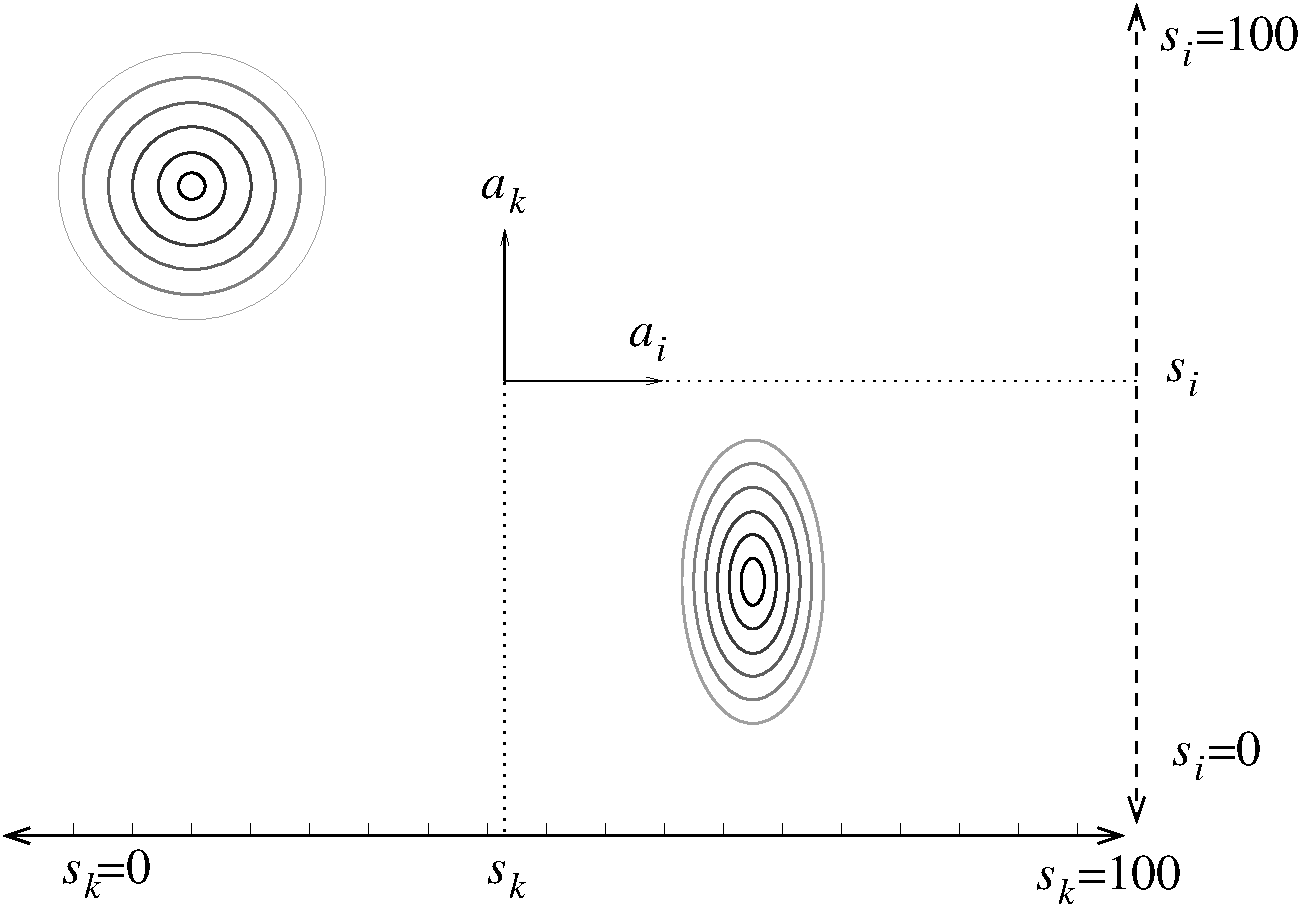
\includegraphics{media/page21figure}}
\end{center}
consider policy learning: execution of $\pi_k(s_k)$ yielding $s^\prime_k$
\end{itemize}

\setlength{\unitlength}{1cm}
\begin{picture}(15,15)
\linespread{1.125}
\selectfont  
\put(7.5,14.7){choice of $a_k$}
\put(8.3,14.25){\vector(-1,-1){3.0}}
\put(8.3,14.25){\vector(1,-1){3.0}}
\put(5.65,13.4){good}
\put(5.65,12.9){$s_i$, $s_j$}
\put(6.7,12.1){$a_k\in\text{Good}$}
\put(6.2,11.5){\underline{$Q(s_k,a_{k1})$}}
%
\put(4.1,10.3){$M_i$}
\put(3.9,9.65){\vector(-1,-1.2){2.0}}
\put(4.6,9.65){\vector(1,-1.2){2.0}}
%
\put(1.7,8.5){same}
\put(1.65,6.5){\circled{A}}
\put(0.8,5.5){$R_t()$ stays same}
%
\put(5.9,8.5){improves}
\put(6.45,6.5){\circled{B}}
\put(5.8,5.5){$R_t()$ increases}
%
\put(9.8,13.4){bad}
\put(9.8,12.9){$s_i$, $s^\prime_i$}
\put(8.8,12.1){$a_k\in\text{Bad}$}
\put(9,11.5){\underline{$Q(s_k,a_{k2})$}}
%
%
\put(10.5,10.3){$M_i$ chooses $a_i$ (store $s_i$, $s_j$, $a_k$)}
\put(11.7,9.65){\vector(-1,-1.2){2.0}}
\put(12.4,9.65){\vector(1,-1.2){2.0}}
%
\put(9,8.5){stays bad}
\put(9.5,6.5){\circled{C}}
\put(8.5,5.5){\parbox[t]{4cm}{$M_i$ can't learn to improve situation}}
\put(8.5,4){$R_t()\text{s}$ stagnate}
%
\put(13.9,8.5){turns max Q(}
\put(14.5,6.5){\circled{D}}
\put(13.5,5.5){\parbox[t]{4cm}{$M_i$ learning to create maximum reward using $a_i$}}
\put(13.5,4){$R_t()$ increases}
%
\qbezier(2,3.5)(2.4,1.9)(4,1.5)
\qbezier(6,3.5)(6.3,2.3)(7,1.75)
\qbezier(10,3.5)(9.7,2.3)(9,1.75)
\qbezier(14.5,3.5)(14.1,1.9)(12.5,1.5)
\put(6,1){\parbox[t]{4cm}{end up in same $s_k^\prime=s_k$, so complete degeneracy}}
\end{picture}

As $t\to\infty$,\begin{minipage}[t]{\linegoal} 
\begin{enumerate}[label=\roman*)]
\item \circled{A} \& \circled{C} will never be selected by $M_k()$
\item if \circled{B}$>$\circled{D} $Q(a_k\in\text{Good},s_k)>Q(a_k\in\text{Bad})$ and then $a_k\in\text{Good}$ will be chosen
\end{enumerate}
\end{minipage}


\newpage

\section*{page 22}

Child convergence rewrite, using time index\\

\setlength{\unitlength}{1cm}
\begin{picture}(15,20)

\put(0.5,20){\parbox[t]{\linegoal}{
$m_1, \ldots, m_\alpha$\\

$m_1$: $(s_i,s_k)$ $\qquad$ pre-existing $s_i=1$, $s_k=1$\\

$m_2$: $a_k=\pi_k(s_k)=(x)$ --- worst case, effects \underline{only} $s_i$, $s_j$,\\

$m_3$: \parbox[t]{\linegoal}{$a_i=\pi_i(s_i,a_k)$\\
$s^\prime_i\leftarrow 2$\\
$s^\prime_k\leftarrow 2$}\\

$m_4$: $Q(s_k,a_k)\leftarrow \text{update}$: $R(s_k,a_k,s^\prime_k)$\\

$m_5$: \parbox[t]{\linegoal}{$Q(s_i,a_k,s_i)\leftarrow \text{update}$: $R(s_i,a_k,a_i,s^\prime_k)$\\
$\hookrightarrow$ update $\pi_i(s_i,a_k)$}\\

so: \framebox[10.5cm][t]{\parbox[t]{10cm}{$m_2$ assumed $\pi(s_i,a_k)(m_3)$ to be  convergent stochastic and monotonic in reward \textbf{???}, which is assured by updating $Q(s_i,a_k,a_i)$ at $m_5$}}\\

$\pi_k(s_k)\rightarrow Q(s_k,a_k)$ $\qquad$ $\pi_i(s_i,a_k)\rightarrow Q(s_k,a_k,s_k)$
}}
\put(0.25,16.85){supposes}
\put(0,17.25){\vector(1,0){0.4}}
\put(0,16.4){\vector(1,0){0.4}}
\put(0,12.4){\line(1,0){0.4}}
\put(0,17.25){\line(0,-1){4.85}}
\end{picture}






\newpage

\section{page 23}

\underline{Bad MDP Decomposition} (worst possible case)\\

\setlength{\unitlength}{1cm}
\begin{picture}(15,12)
\linespread{1.125}
\selectfont  
\put(1,4){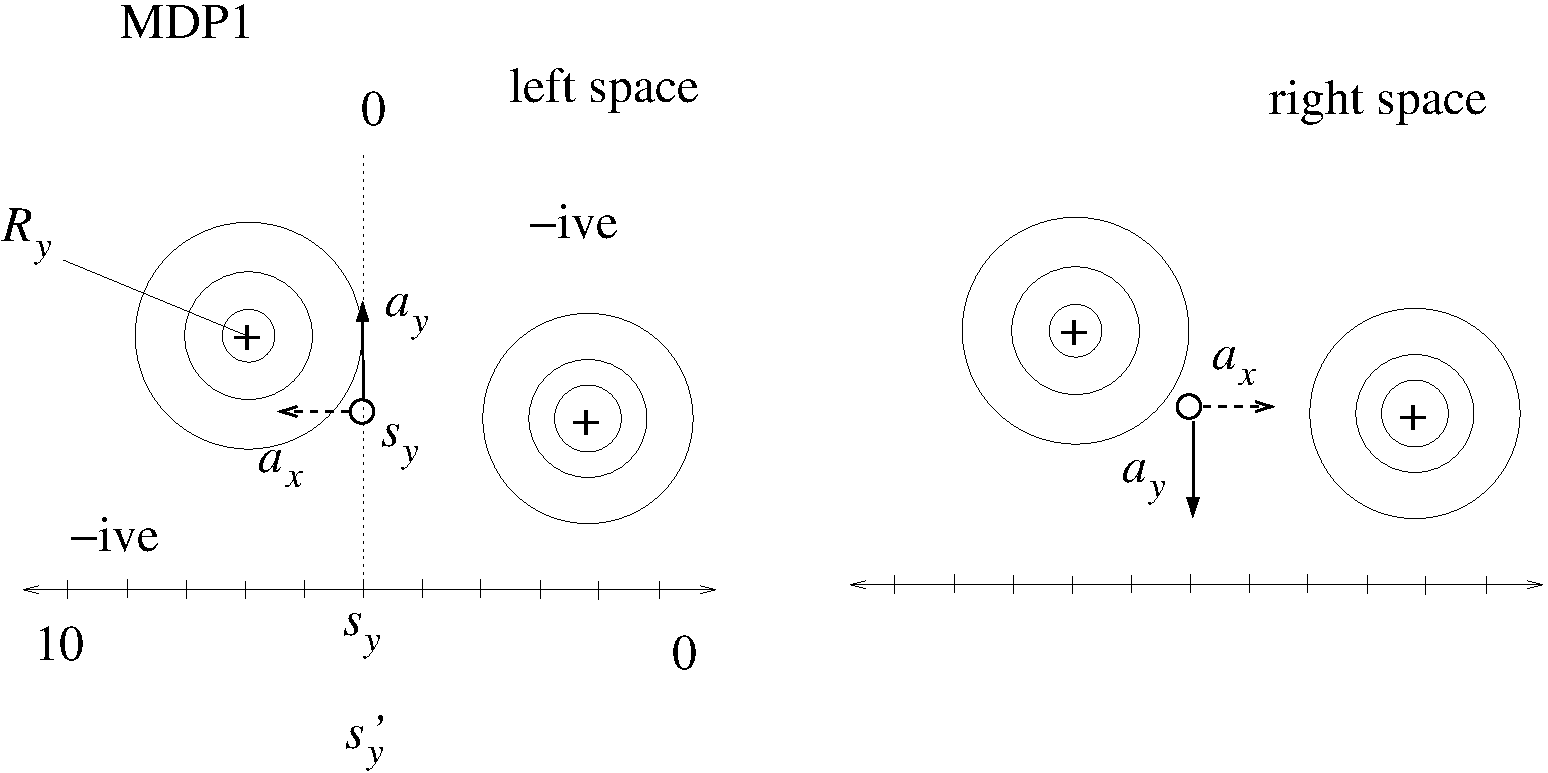
\includegraphics[scale=0.5]{media/page23figure.pdf}}


\put(9.5,4){\parbox[t]{4cm}{result -- no impact on reward directly}}

\put(9.5,2){\parbox[t]{4cm}{\underline{Latent reality}: move system into a position of advantage through actions}}

\put(1.5,3){\framebox[4.25cm][t]{\parbox[t]{4cm}{example of `'bad MDP'' which, in isolation, is useless}}}

\end{picture}

ways to understand:
$\qquad$ \begin{minipage}[t]{\linegoal}
\begin{enumerate}[label=\arabic*)]
\item analyze actions of subsystem

\item analyze effectiveness of subsystem\\
$\qquad\hookrightarrow$ Do until ave coordination
\end{enumerate}
\end{minipage}\\

only ability: \parbox[t]{\linegoal}{coordinate acting with subsystem, s.t., an understanding of the relationship of your action \& subsystem action arises}


\end{document}
